\documentclass[12pt]{article}
\usepackage{geometry}
\geometry{margin=2cm}
\geometry{letterpaper}

\newcommand{\hide}[1]{}
\newcommand{\exerciseoneb}{\texttt{exercise1b.py}\;}
\newcommand{\exerciseonec}{\texttt{exercise1c.py}\;}
\newcommand{\exerciseoned}{\texttt{exercise1d.py}\;}
\newcommand{\exerciseonee}{\texttt{exercise1e.py}\;}
\newcommand{\exercisetwoaone}{\texttt{exercise2a\_network1.py}\;}
\newcommand{\exercisetwoatwo}{\texttt{exercise2a\_network2.py}\;}
\newcommand{\exercisetwoathree}{\texttt{exercise2a\_network3.py}\;}
\newcommand{\exercisetwob}{\texttt{exercise2b.py}\;}

\renewcommand\thesubsection{\thesection.\alph{subsection}}

\usepackage{xcolor}
\usepackage{url}
\usepackage{hyperref}
\usepackage{enumitem}
\usepackage{array}
\usepackage{mathtools}
\usepackage{graphicx}
\usepackage[labelfont=bf]{caption}
\usepackage{subcaption}
\usepackage{ textcomp }

\hide{
\usepackage{amscd}
\usepackage{amsfonts}
\usepackage{amsmath}
\usepackage{amssymb}
\usepackage{amsthm}
\usepackage{cases}		 
\usepackage{cutwin}
\usepackage{enumerate}
\usepackage{epstopdf}
\usepackage{graphicx}
\usepackage{ifthen}
\usepackage{lipsum}
\usepackage{mathrsfs}	
\usepackage{multimedia}
\usepackage{wrapfig}
}

\newcommand{\itemlist}[1]{\begin{itemize}#1\end{itemize}}
\newcommand{\enumlist}[1]{\begin{enumerate}#1\end{enumerate}}
\newcommand{\desclist}[1]{\begin{description}#1\end{description}}

\title {Crash Course Deep Learning - Assignment 2}
\author{Instructor:  Prof. Alexander Sch\"onhuth \\ Submitted by: Jan Gerrit H\"olting \\ Student ID: 6570518 \\ Universiteit Utrecht}
\date{}

\begin{document}
\maketitle
In this report, we will investigate the performance of convolutional neural networks in recognising handwritten digits. The report can be seen as an extension to \cite{JG}, where basic neural networks (NN) have been applied to the same problem. The best accuracy any conventional neural network achieved was at 98\% within approximately 20 minutes of training and can be found in Section 1b of \cite{JG}. In this report, we will therefore try to improve the performance and efficiency of handwritten digit recognition with the use of convolutional neural networks (CNN). 

The test data set for the neural network will again be the MNIST database of handwritten digits (see \cite{MNIST}) containing 60,000 training examples as well as 10,000 test examples. The experimental results have been obtained using the accompanying Python implementation which in turn uses Google's open-source machine learning platform TensorFlow 2 (see \cite{TensorFlow}). All the code that has been used can be found in the GitHub repository \cite{JGitHub}. \\


\noindent \textbf{General setup:} \\

Some parameters of the neural network will remain constant throughout the following experiments. For more information on the interpretation of the parameters as well as the methods used, the reader is asked to consult Nielsen's \textit{Neural Networks and Deep Learning} \cite{Nielsen} for an informal or Goodfellow et al.s' \textit{Deep Learning} \cite{Goodfellow} for a more formal introduction. We will use 50 epochs, a batch size of 100 while iterating through the example data and a standard gradient descent optimizer with a learning rate of 0.05. This means that we will deviate from \cite{JG} by choosing a much smaller learning rate (0.05 as compared to 0.5 in the earlier report). Furthermore, we will for each tested architecture only use one split of training, validation and test data and therefore refrain from cross-validation. As we will see, this improves efficiency while still achieving high accuracy of the chosen models. In the output layer we will use cross entropy as the loss function with softmax activation. All convolutional hidden layers will use ReLU as activation function while all fully connected hidden layers will use the sigmoid function as the activation function. Furthermore, the number 6570518 is used as a seed for all random variable initialisation.


\newpage
\section{Exercises}
\subsection{}\label{sec:exercise1a}

In this first part of the report, we will discuss a small but essential difference between conventional and convolutional neural networks, namely their differing approach in handling input data and data that is passed in-between layers. In the code for all of the following CNNs (see assignments/assignment2 in \cite{JGitHub}) we will see that the network's input is reshaped as 
$$ \texttt{x\_train = x\_train.reshape(x\_train.shape[0], img\_rows, img\_cols, 1)
}$$ 
thus differing to the method 
$$ \texttt{x\_train = x\_train.reshape((-1, img\_rows*img\_cols))} $$ 
used in the earlier report \cite{JG}. 

Now the second command flattens the image, because fully connected NNs expect a vector as input (every layer's weights and biases are represented by a matrix), and all pixels are treated equally (there is no bundling of pixels based on their location in the vector). The second command returns a matrix representing the pixels which will be iterated through by the network automatically (in TensorFlow Keras). On a high level (not taking into account the actual memory structure and access), this makes the handling much easier and more intuitive than having to handle neighbourhood pixels with their indices in a flat vector. This is important because in CNNs, local environments of a pixel are taking into account. The 1 at the end of the first command indicates that we are handling a one-dimensional image in the sense that our input is a greyscale image instead of one that is RGB encoded. For an RGB encoded image, the 1 would be replaced by a 3. The application of a filter to an input image represented by a matrix of (grey-scale) values can be seen in Figure \ref{fig:exercise1a}.


\begin{figure}[ht]
\centering
   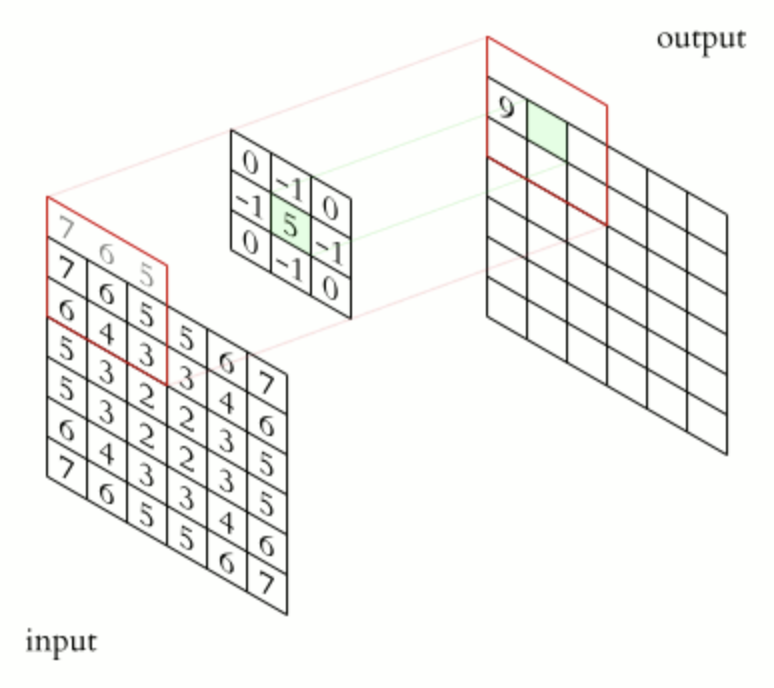
\includegraphics[scale=0.6]{graphics/CNNs.png}
    \caption{The working of a filter applied to an input image represented as a matrix of (grey-scale) values. Screenshot taken from Michael Plotke's animation on the German entry for CNNs on wikipedia, see \cite{Plotke}.}
    \label{fig:exercise1a}
\end{figure}

\subsection{}\label{sec:exercise1b}
As a first exercise in understanding the structure of CNNs, we will consider the following network: \\
\begin{enumerate}[nolistsep]
\item Input layer
\item Convolution layer with a 5\texttimes5 filter and 6 output channels, stride 1, padding, followed by activation function ReLU
\item Max pooling layer with a 2\texttimes2 filter and stride 2\texttimes2, zero padding
\item Fully connected layer with 128 nodes, sigmoid as activation function
\item Output layer.\\
\end{enumerate}

\noindent The Python implementation for this model can be found in \exerciseoneb in assignments/assignment2 in \cite{JGitHub}. 


\subsection{}\label{sec:exercise1c}
Now the internal structure of the network (the output shapes of each layer) can be requested as a concise summary with the Keras command \texttt{model.summary()}. For the model proposed in \ref{sec:exercise1b}, the output can be seen in Figure \ref{fig:exercise1c}

\begin{figure}[ht]
\centering
   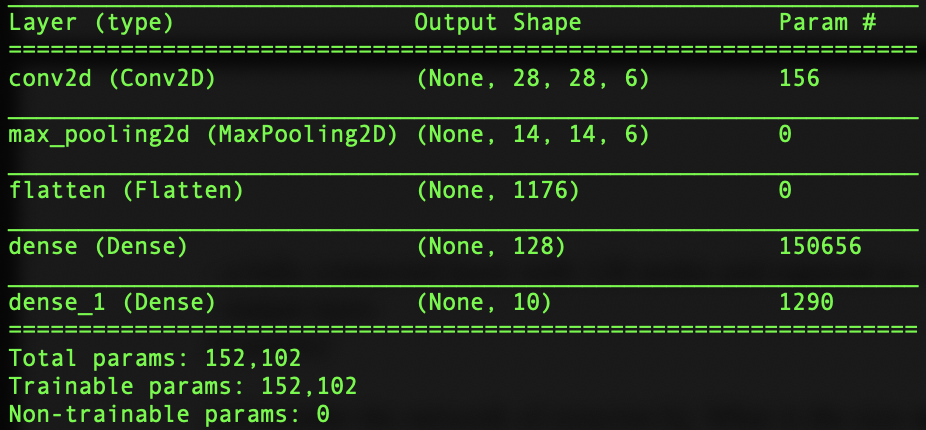
\includegraphics[scale=0.7]{graphics/model1b.png}
    \caption{The internal data structure of the CNN proposed in Section \ref{sec:exercise1b}, created by the Keras command \texttt{model.summary()}.}
    \label{fig:exercise1c}
\end{figure}

The input images of the MNIST data set are of dimension 28\texttimes28. Since in Section \ref{sec:exercise1b} we decided to use padding in the (first,) convolutional layer with 6 output channels, we can observe that the output of that layer is again 28\texttimes28\texttimes6: the third dimension of 6 is a result of the choice of output channels, the 28\texttimes28 dimensions are kept because we use padding and a stride length of 1. Hence, each pixel will be considered as the center of a 5\texttimes5 local reference field and therefore contributes an output value, and we don't loose any dimensions in the output of this first layer. Something similiar (though with 3\texttimes3 filters) can be observed in Figure \ref{fig:exercise1a} where the padding of the image is chosen to be the closest pixel on the border of the image instead of 0. 

The MaxPooling layer on the other hand significantly decreases the output dimensions: here we find dimensions of 14\texttimes14\texttimes6, the 6 again resulting from the use of 6 output channels. The dimensions fo 14\texttimes14 are a consequence of using no padding as well as a stride length of 2 in both directions: each entry of the output of one channel will only be used once for pooling and no padding is used; the stride and filter dimensions of 2\texttimes2 therefore halve each dimension.


\subsection{}\label{sec:exercise1d}

We can observe the effect that padding has on the output dimensions of the convolutional layer by removing it from the first layer. The \texttt{model.summary()} for this CNN can be seen in Figure \ref{fig:exercise1d}.

\begin{figure}[ht]
\centering
   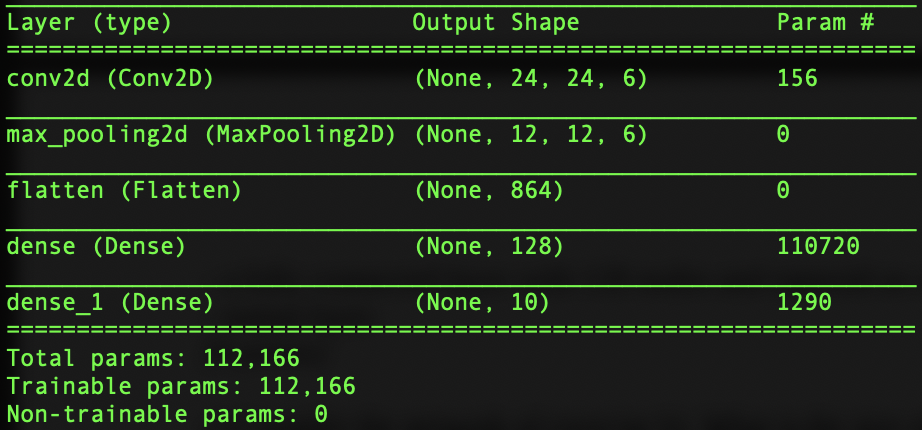
\includegraphics[scale=0.7]{graphics/model1d.png}
  \caption{The internal data structure of the CNN proposed in Section \ref{sec:exercise1b} without padding in the convolutional layer, created by the Keras command \texttt{model.summary()}.}
    \label{fig:exercise1d}
\end{figure}

As we can see, the output shape of the first layer in this example only is 24\texttimes24\texttimes6 as compared to 28\texttimes28\texttimes6 in \ref{sec:exercise1c}. Since no padding is used in this case, only the pixels with coordinates $(i,j), i, j \in [3, 26]$ (counting from 1) occur as centres of a local reference field (LRF) of size 5\texttimes5. The output channel dimension of 6 remains the same.


\subsection{}\label{sec:exercise1e}
If we now change the stride size of the first layer in the model of Section \ref{sec:exercise1b} (thus keeping the padding), we can observe the following changes to the output dimensions of the first layer. 

\begin{figure}[ht]
\centering
   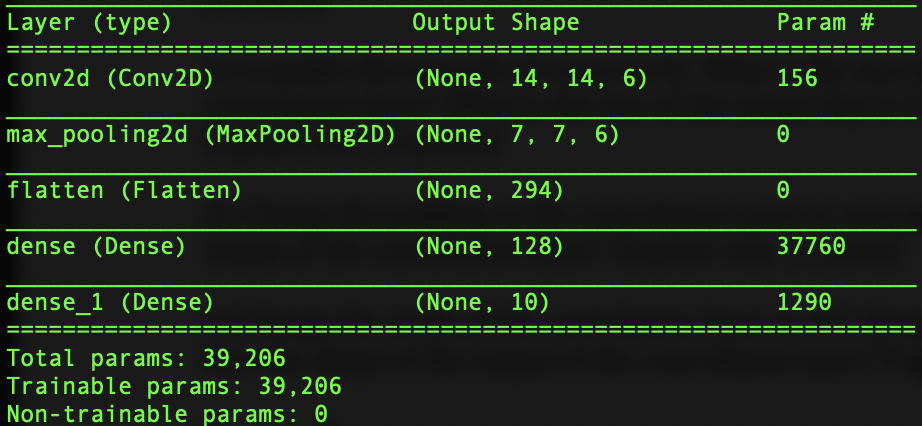
\includegraphics[scale=0.7]{graphics/model1e.png}
    \caption{The internal data structure of the CNN proposed in Section \ref{sec:exercise1b} with stride size 2 in each direction in the convolutional layer, created by the Keras command \texttt{model.summary()}.}
    \label{fig:exercise1e}
\end{figure}

In Figure \ref{fig:exercise1e} we can see that the output shape of the first layer has now changed to 14\texttimes14\texttimes6 even though we are still using padding. In this case, every pixel with coordinates $(i,j), i, j \in [1,28]$ (counting from 1) where both $i$ and $j$ are uneven is considered as the centre of a LRF because of the stride size. We are therefore again halving the output dimensions of the first layer. 


\section{Evaluating different CNN architectures}
\subsection{}\label{sec:exercise2a}
Similar to \cite{JG}, we will use this second part of the report to evaluate the performance of different architectures of CNNs. All of the architectures tested in the following will have at least two convolutional layers, two max pooling layers and one fully connected layer. The three architectures can be viewed in detail in Table \ref{tab:exercise2a_models}.

\begin{table}[ht]
    \centering
    \begin{tabular}{p{5.5cm}|p{5.5cm}|p{5.5cm}}
         \multicolumn{1}{c|}{\textbf{Model 1}} & \multicolumn{1}{c|}{\textbf{Model 2}} & \multicolumn{1}{c}{\textbf{Model 3}} \\ \hline 
\begin{enumerate}[nolistsep, leftmargin=*]
\item Input layer
\item Convolution layer, 5\texttimes5 filter, 16 output channels, stride 1, padding, activation function ReLU
\item Max pooling layer, 2\texttimes2 filter, stride 2, zero padding
\item Convolution layer, 3\texttimes3 filter, 32 output channels, stride 1, padding, activation function ReLU
\item Max pooling layer, 2\texttimes2 filter, stride 2, zero padding
\item Fully connected layer, 128 nodes, sigmoid as activation function
\item Output layer
\end{enumerate} & 

\begin{enumerate}[nolistsep, leftmargin=*]
\item Input layer
\item Convolution layer, 5\texttimes5 filter, 16 output channels, stride 1, padding, activation function ReLU
\item Max pooling layer, 2\texttimes2 filter, stride 2, zero padding
\item Convolution layer, 3\texttimes3 filter, 32 output channels, stride 1, padding, activation function ReLU
\item Max pooling layer, 2\texttimes2 filter, stride 2, zero padding
\item Fully connected layer, 256 nodes, sigmoid as activation function
\item Fully connected layer, 128 nodes, sigmoid as activation function
\item Output layer
\end{enumerate}
 & 
 \begin{enumerate}[nolistsep, leftmargin=*]
\item Input layer
\item Convolution layer, 7\texttimes7 filter, 16 output channels, stride 1, padding, activation function ReLU
\item Max pooling layer, 2\texttimes2 filter, stride 2, zero padding
\item Convolution layer, 5\texttimes5 filter, 32 output channels, stride 1, padding, activation function ReLU
\item Max pooling layer, 2\texttimes2 filter, stride 2, zero padding
\item Fully connected layer, 256 nodes, sigmoid as activation function
\item Fully connected layer, 128 nodes, sigmoid as activation function
\item Output layer
\end{enumerate}
    \end{tabular}
     \caption{Three different architectures of CNNs.}
        \label{tab:exercise2a_models}
\end{table}

\noindent The implementation of these models can be found in \texttt{exercise2a.py}. The resulting performance values of the three different architectures can be seen in Table \ref{tab:exercise2a_values}. Again, the validation loss and efficiency has been used to determine the best performing model. Additionally, the loss over epochs for all three models can be observed in Figure \ref{fig:exercise2a_loss_epochs}.

\begin{figure}[ht]
\centering
   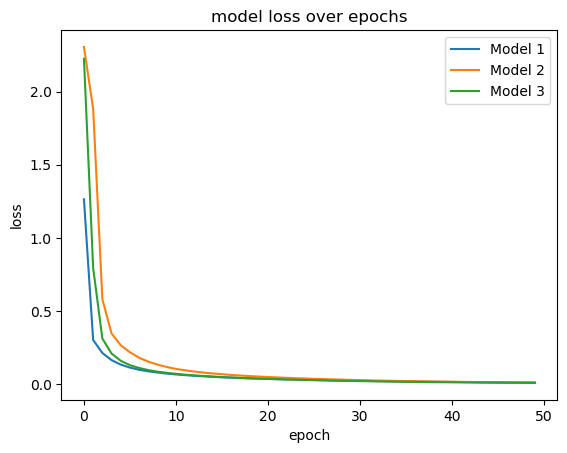
\includegraphics[scale=0.7]{graphics/loss_over_epochs_exercise_2a.png}
    \caption{Plot of the evolution of loss over 50 epochs of training the three CNN architectures proposed in Table \ref{tab:exercise2a_models}.}
    \label{fig:exercise2a_loss_epochs}
\end{figure}

\begin{table}[ht]
    \centering
    \begin{tabular}{c|c|c|c}
        \textbf{Model}              & \textbf{Validation loss} & \textbf{Total parameters} &   \textbf{Time (min:sec)} \\ \hline
        1 &  0.04368 & 207,178 &  13:38           \\  
        3 &  0.04466 & 440,906 & 14:35           \\ 
        2 &  0.04151 & 449,482 & 19:53           \\
    \end{tabular}
     \caption{Comparing different NN architectures with regard to average validation loss, accuracy on the test data and time taken for training (in minutes).}
        \label{tab:exercise2a_values}
\end{table}

\noindent From Table \ref{tab:exercise2a_values} we observe that Model 3 is the best-performing, with regard to its loss value on the validation data but not with regard to its timing; models 1 and 2 both achieve similar validation loss and timing results. The timing values also correspond to the number of trainable parameters, of which Model 3 has the most (these can conveniently be requested through \texttt{model.summary()}). Overall, however, we can observe in Figure \ref{fig:exercise2a_loss_epochs} that despite initial differences in training loss, all three models converge to similar values after approximately 25 epochs of training. Testing Model 3 on the separate test set (remember that the MNIST data base is split into 60,000 training images and 10,000 test images) leads to an accuracy of 98.96\%. We can therefore conclude that this model outperforms the best NN in \cite{JG} (98\% accuracy after approximately 20 minutes of training) with respect to accuracy at a similar training time.


\subsection{}

The previous section suggested that having convolutional rather than fully connected layers in a neural network is more efficient both with respect to accuracy and training time. In this section, we will therefore test whether a deeper but lighter network, i.e. one with one more convolutional layer but less trainable parameters, can achieve similar performance results while requiring the same or less training time. The accompanying Python code can be found in \exercisetwob. We will leave the common parameters described in the introduction the same in order to achieve some comparability of the hyperparemeters. The chosen model has the following architecture: \\

\begin{enumerate}[nolistsep]
\item Input layer
\item Convolution layer with a 4\texttimes4 filter and 32 output channels, stride 2, padding, followed by activation function ReLU
\item Max pooling layer with a 2\texttimes2 filter and stride 2\texttimes2, zero padding
\item Convolution layer with a 4\texttimes4 filter and 16 output channels, stride 1, padding, followed by activation function ReLU
\item Max pooling layer with a 2\texttimes2 filter and stride 2\texttimes2, zero padding
\item Convolution layer with a 2\texttimes2 filter and 9 output channels, stride 1, padding, followed by activation function ReLU
\item Max pooling layer with a 2\texttimes2 filter and stride 2\texttimes2, zero padding
\item Fully connected layer with 128 nodes, sigmoid as activation function
\item Output layer.\\
\end{enumerate}

\noindent The \texttt{model.summary()} can be found in Figure \ref{fig:exercise2b}; as we can see, the number of trainable parameters is at only 2.5\% of those of Model 3 of Section \ref{sec:exercise2a}. 

\begin{figure}[ht]
\centering
   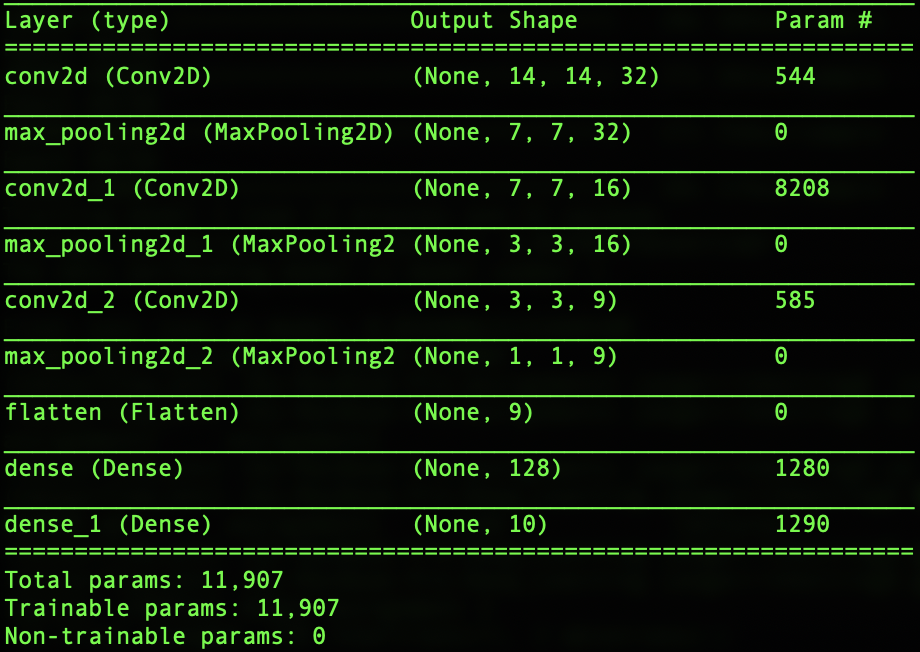
\includegraphics[scale=0.7]{graphics/model2b.png}
    \caption{The internal data structure of the CNN proposed in Section \ref{sec:exercise1b}, created by the Keras command \texttt{model.summary()}.}
    \label{fig:exercise2b}
\end{figure}

Now to evaluate this model's performance, we will again consider the final accuracy on the test data. In general, it is advised to use as much training data as possible to fit the model and hence to refrain from using a training, validation and test dataset (split into 48,000, 12,000 and 10,000 images) and instead use a simply training and test data split and use the additional 12,000 validation images for training. Since we are not interested in further tuning the hyperparameters and we aborting the cross-validation after just one fold, it is not necessary to use a separate validation data set. Using only training and test data results in 14 minutes of training and an accuracy 98.57\%. Even though the model has significantly less parameters to train, it does not take proportionally less time for training (roughly 14 minutes) as compared to Model 3 from Section \ref{sec:exercise2a} and achieves slightly worse accuracy on the test data. If storage space is of any concern, then going for this deep and light architecture might be of advantage; however, on modern computers, training parameters of roughly 400,000 should be no reason for concern. Altogether, Model 3 therefore remains the best tested architecture of this report with a test accuracy of 98.96\% after 14 minutes of training. 


\newpage
\section{Conclusion}

To conclude this report on the use of (C)NNs for handwritten digit recognition of the MNIST data set, we note that the use of CNNs significantly outperformed fully connected neural networks. We have seen that with comparatively little training time and a simple CNN architecture with just five layers, an accuracy of 98.96\% correctly recognised digits could be achieved. 

\bibliographystyle{alphadin}
\bibliography{DL_2}
\end{document}